\documentclass[twoside]{book}

% Packages required by doxygen
\usepackage{fixltx2e}
\usepackage{calc}
\usepackage{doxygen}
\usepackage[export]{adjustbox} % also loads graphicx
\usepackage{graphicx}
\usepackage[utf8]{inputenc}
\usepackage{makeidx}
\usepackage{multicol}
\usepackage{multirow}
\PassOptionsToPackage{warn}{textcomp}
\usepackage{textcomp}
\usepackage[nointegrals]{wasysym}
\usepackage[table]{xcolor}

% Font selection
\usepackage[T1]{fontenc}
\usepackage[scaled=.90]{helvet}
\usepackage{courier}
\usepackage{amssymb}
\usepackage{sectsty}
\renewcommand{\familydefault}{\sfdefault}
\allsectionsfont{%
  \fontseries{bc}\selectfont%
  \color{darkgray}%
}
\renewcommand{\DoxyLabelFont}{%
  \fontseries{bc}\selectfont%
  \color{darkgray}%
}
\newcommand{\+}{\discretionary{\mbox{\scriptsize$\hookleftarrow$}}{}{}}

% Page & text layout
\usepackage{geometry}
\geometry{%
  a4paper,%
  top=2.5cm,%
  bottom=2.5cm,%
  left=2.5cm,%
  right=2.5cm%
}
\tolerance=750
\hfuzz=15pt
\hbadness=750
\setlength{\emergencystretch}{15pt}
\setlength{\parindent}{0cm}
\setlength{\parskip}{3ex plus 2ex minus 2ex}
\makeatletter
\renewcommand{\paragraph}{%
  \@startsection{paragraph}{4}{0ex}{-1.0ex}{1.0ex}{%
    \normalfont\normalsize\bfseries\SS@parafont%
  }%
}
\renewcommand{\subparagraph}{%
  \@startsection{subparagraph}{5}{0ex}{-1.0ex}{1.0ex}{%
    \normalfont\normalsize\bfseries\SS@subparafont%
  }%
}
\makeatother

% Headers & footers
\usepackage{fancyhdr}
\pagestyle{fancyplain}
\fancyhead[LE]{\fancyplain{}{\bfseries\thepage}}
\fancyhead[CE]{\fancyplain{}{}}
\fancyhead[RE]{\fancyplain{}{\bfseries\leftmark}}
\fancyhead[LO]{\fancyplain{}{\bfseries\rightmark}}
\fancyhead[CO]{\fancyplain{}{}}
\fancyhead[RO]{\fancyplain{}{\bfseries\thepage}}
\fancyfoot[LE]{\fancyplain{}{}}
\fancyfoot[CE]{\fancyplain{}{}}
\fancyfoot[RE]{\fancyplain{}{\bfseries\scriptsize Generated by Doxygen }}
\fancyfoot[LO]{\fancyplain{}{\bfseries\scriptsize Generated by Doxygen }}
\fancyfoot[CO]{\fancyplain{}{}}
\fancyfoot[RO]{\fancyplain{}{}}
\renewcommand{\footrulewidth}{0.4pt}
\renewcommand{\chaptermark}[1]{%
  \markboth{#1}{}%
}
\renewcommand{\sectionmark}[1]{%
  \markright{\thesection\ #1}%
}

% Indices & bibliography
\usepackage{natbib}
\usepackage[titles]{tocloft}
\setcounter{tocdepth}{3}
\setcounter{secnumdepth}{5}
\makeindex

% Hyperlinks (required, but should be loaded last)
\usepackage{ifpdf}
\ifpdf
  \usepackage[pdftex,pagebackref=true]{hyperref}
\else
  \usepackage[ps2pdf,pagebackref=true]{hyperref}
\fi
\hypersetup{%
  colorlinks=true,%
  linkcolor=blue,%
  citecolor=blue,%
  unicode%
}

% Custom commands
\newcommand{\clearemptydoublepage}{%
  \newpage{\pagestyle{empty}\cleardoublepage}%
}

\usepackage{caption}
\captionsetup{labelsep=space,justification=centering,font={bf},singlelinecheck=off,skip=4pt,position=top}

%===== C O N T E N T S =====

\begin{document}

% Titlepage & ToC
\hypersetup{pageanchor=false,
             bookmarksnumbered=true,
             pdfencoding=unicode
            }
\pagenumbering{roman}
\begin{titlepage}
\vspace*{7cm}
\begin{center}%
{\Large My Project }\\
\vspace*{1cm}
{\large Generated by Doxygen 1.8.11}\\
\end{center}
\end{titlepage}
\clearemptydoublepage
\tableofcontents
\clearemptydoublepage
\pagenumbering{arabic}
\hypersetup{pageanchor=true}

%--- Begin generated contents ---
\chapter{Class Index}
\section{Class List}
Here are the classes, structs, unions and interfaces with brief descriptions\+:\begin{DoxyCompactList}
\item\contentsline{section}{\hyperlink{structnode}{node} }{\pageref{structnode}}{}
\item\contentsline{section}{\hyperlink{structnode1}{node1} }{\pageref{structnode1}}{}
\item\contentsline{section}{\hyperlink{structnode__info}{node\+\_\+info} }{\pageref{structnode__info}}{}
\end{DoxyCompactList}

\chapter{File Index}
\section{File List}
Here is a list of all files with brief descriptions\+:\begin{DoxyCompactList}
\item\contentsline{section}{\hyperlink{Lab1_8c}{Lab1.\+c} }{\pageref{Lab1_8c}}{}
\end{DoxyCompactList}

\chapter{Class Documentation}
\hypertarget{structPlayer}{}\section{Player Struct Reference}
\label{structPlayer}\index{Player@{Player}}
\subsection*{Public Member Functions}
\begin{DoxyCompactItemize}
\item 
\hyperlink{structPlayer_acc54f586b782d5283245d4fc8a7e033c}{Player} (int player\+Id, std\+::string player\+Name)
\item 
void \hyperlink{structPlayer_afa7a00da55d6cc124d6b3351dba72f4a}{add\+Points} (int p)
\end{DoxyCompactItemize}
\subsection*{Public Attributes}
\begin{DoxyCompactItemize}
\item 
int \hyperlink{structPlayer_a05e05f3a23de78da7ec032ec2bcf8c6c}{id}
\item 
int \hyperlink{structPlayer_adf0398ea8c1f29175204508ab642b64e}{points}
\item 
std\+::string \hyperlink{structPlayer_af9c920fabaafdeb7961a645315b521ff}{name}
\end{DoxyCompactItemize}


\subsection{Constructor \& Destructor Documentation}
\index{Player@{Player}!Player@{Player}}
\index{Player@{Player}!Player@{Player}}
\subsubsection[{\texorpdfstring{Player(int player\+Id, std\+::string player\+Name)}{Player(int playerId, std::string playerName)}}]{\setlength{\rightskip}{0pt plus 5cm}Player\+::\+Player (
\begin{DoxyParamCaption}
\item[{int}]{player\+Id, }
\item[{std\+::string}]{player\+Name}
\end{DoxyParamCaption}
)\hspace{0.3cm}{\ttfamily [inline]}}\hypertarget{structPlayer_acc54f586b782d5283245d4fc8a7e033c}{}\label{structPlayer_acc54f586b782d5283245d4fc8a7e033c}

\begin{DoxyCode}
11                                                :
12             \hyperlink{structPlayer_a05e05f3a23de78da7ec032ec2bcf8c6c}{id}(playerId), \hyperlink{structPlayer_af9c920fabaafdeb7961a645315b521ff}{name}(playerName)
13     \{
14         \hyperlink{structPlayer_adf0398ea8c1f29175204508ab642b64e}{points} = 0;
15     \}
\end{DoxyCode}


\subsection{Member Function Documentation}
\index{Player@{Player}!add\+Points@{add\+Points}}
\index{add\+Points@{add\+Points}!Player@{Player}}
\subsubsection[{\texorpdfstring{add\+Points(int p)}{addPoints(int p)}}]{\setlength{\rightskip}{0pt plus 5cm}void Player\+::add\+Points (
\begin{DoxyParamCaption}
\item[{int}]{p}
\end{DoxyParamCaption}
)\hspace{0.3cm}{\ttfamily [inline]}}\hypertarget{structPlayer_afa7a00da55d6cc124d6b3351dba72f4a}{}\label{structPlayer_afa7a00da55d6cc124d6b3351dba72f4a}

\begin{DoxyCode}
16                           :
17     \{
18         \hyperlink{structPlayer_adf0398ea8c1f29175204508ab642b64e}{points} += p;
19     \}
\end{DoxyCode}


\subsection{Member Data Documentation}
\index{Player@{Player}!id@{id}}
\index{id@{id}!Player@{Player}}
\subsubsection[{\texorpdfstring{id}{id}}]{\setlength{\rightskip}{0pt plus 5cm}int Player\+::id}\hypertarget{structPlayer_a05e05f3a23de78da7ec032ec2bcf8c6c}{}\label{structPlayer_a05e05f3a23de78da7ec032ec2bcf8c6c}
\index{Player@{Player}!name@{name}}
\index{name@{name}!Player@{Player}}
\subsubsection[{\texorpdfstring{name}{name}}]{\setlength{\rightskip}{0pt plus 5cm}std\+::string Player\+::name}\hypertarget{structPlayer_af9c920fabaafdeb7961a645315b521ff}{}\label{structPlayer_af9c920fabaafdeb7961a645315b521ff}
\index{Player@{Player}!points@{points}}
\index{points@{points}!Player@{Player}}
\subsubsection[{\texorpdfstring{points}{points}}]{\setlength{\rightskip}{0pt plus 5cm}int Player\+::points}\hypertarget{structPlayer_adf0398ea8c1f29175204508ab642b64e}{}\label{structPlayer_adf0398ea8c1f29175204508ab642b64e}


The documentation for this struct was generated from the following file\+:\begin{DoxyCompactItemize}
\item 
\hyperlink{Iterator_8cpp}{Iterator.\+cpp}\end{DoxyCompactItemize}

\chapter{File Documentation}
\hypertarget{Iterator_8cpp}{}\section{Iterator.\+cpp File Reference}
\label{Iterator_8cpp}\index{Iterator.\+cpp@{Iterator.\+cpp}}
{\ttfamily \#include $<$iostream$>$}\\*
{\ttfamily \#include $<$string$>$}\\*
{\ttfamily \#include $<$iterator$>$}\\*
{\ttfamily \#include $<$algorithm$>$}\\*
Include dependency graph for Iterator.\+cpp\+:
\nopagebreak
\begin{figure}[H]
\begin{center}
\leavevmode
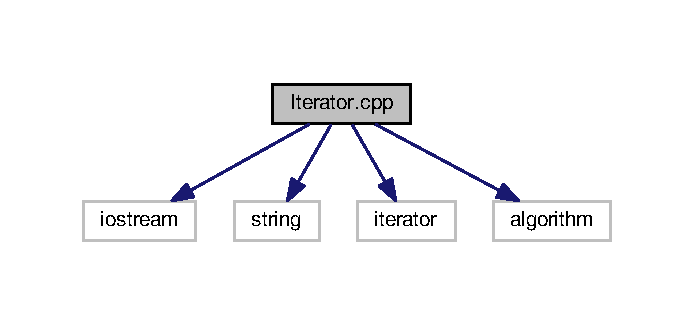
\includegraphics[width=333pt]{Iterator_8cpp__incl}
\end{center}
\end{figure}
\subsection*{Classes}
\begin{DoxyCompactItemize}
\item 
struct \hyperlink{structPlayer}{Player}
\end{DoxyCompactItemize}
\subsection*{Functions}
\begin{DoxyCompactItemize}
\item 
int \hyperlink{Iterator_8cpp_ae66f6b31b5ad750f1fe042a706a4e3d4}{main} ()
\end{DoxyCompactItemize}


\subsection{Function Documentation}
\index{Iterator.\+cpp@{Iterator.\+cpp}!main@{main}}
\index{main@{main}!Iterator.\+cpp@{Iterator.\+cpp}}
\subsubsection[{\texorpdfstring{main()}{main()}}]{\setlength{\rightskip}{0pt plus 5cm}int main (
\begin{DoxyParamCaption}
{}
\end{DoxyParamCaption}
)}\hypertarget{Iterator_8cpp_ae66f6b31b5ad750f1fe042a706a4e3d4}{}\label{Iterator_8cpp_ae66f6b31b5ad750f1fe042a706a4e3d4}

\begin{DoxyCode}
23 \{
24     std::list<Player> listofPlayers =
25     \{ \hyperlink{structPlayer}{Player}(22, \textcolor{stringliteral}{"Sid"}), \hyperlink{structPlayer}{Player}(3, \textcolor{stringliteral}{"Laura"}), \hyperlink{structPlayer}{Player}(43, \textcolor{stringliteral}{"Riti"}), 
      \hyperlink{structPlayer}{Player}(30,
26             \textcolor{stringliteral}{"Angel"}), \hyperlink{structPlayer}{Player}(2, \textcolor{stringliteral}{"Laura"}) \};
27  
28     std::cout << \textcolor{stringliteral}{"*******Iterate std::list using Iterators*******"} << std::endl;
29  
30 \textcolor{comment}{//Create an iterator of std::list}
31     std::list<Player>::iterator it;
32  
33 \textcolor{comment}{// Make iterate point to begining and incerement it one by one till it reaches the end of list.}
34     \textcolor{keywordflow}{for} (it = listofPlayers.begin(); it != listofPlayers.end(); it++)
35     \{
36         \textcolor{comment}{// Access the object through iterator}
37         \textcolor{keywordtype}{int} \textcolor{keywordtype}{id} = it->\hyperlink{structPlayer_a05e05f3a23de78da7ec032ec2bcf8c6c}{id};
38         std::string name = it->name;
39         it->addPoints(2);
40  
41         \textcolor{comment}{//Print the contents}
42         std::cout << \textcolor{keywordtype}{id} << \textcolor{stringliteral}{" :: "} << name << std::endl;
43  
44     \}
45  
46     std::cout
47             << \textcolor{stringliteral}{"*******Iterate std::list using for\_each and c++11's Lambda function *********"}
48             << std::endl;
49  
50     std::for\_each(listofPlayers.begin(), listofPlayers.end(),
51             [](\textcolor{keyword}{const} \hyperlink{structPlayer}{Player} & player)
52             \{
53                 \textcolor{comment}{//Print the contents}
54                 std::cout<<player.id<< \textcolor{stringliteral}{" :: "}<<player.name<<std::endl;
55                 player.addPoints(5);
56             \});
57  
58     std::cout
59             << \textcolor{stringliteral}{"*******Iterate std::list using c++11 Range Based For Loop *********"}
60             << std::endl;
61  
62     \textcolor{keywordflow}{for} (\textcolor{keyword}{const} \hyperlink{structPlayer}{Player} & player : listofPlayers)
63     \{
64         std::cout << player.id << \textcolor{stringliteral}{" :: "} << player.name << std::endl;
65         player.addPoints(3);
66     \}
67  
68     std::cout
69             << \textcolor{stringliteral}{"*******Iterate std::list in backwords using Iterators *********"}
70             << std::endl;
71  
72     \textcolor{comment}{//Create a reverse iterator of std::list}
73     std::list<Player>::reverse\_iterator revIt;
74  
75     \textcolor{comment}{// Make iterate point to begining and incerement it one by one till it reaches the end of list.}
76     \textcolor{keywordflow}{for} (revIt = listofPlayers.rbegin(); revIt != listofPlayers.rend(); revIt++)
77     \{
78         \textcolor{comment}{// Access the object through iterator}
79         \textcolor{keywordtype}{int} \textcolor{keywordtype}{id} = revIt->id;
80         std::string name = revIt->name;
81         rivIt->addPoints(9);
82  
83         \textcolor{comment}{//Print the contents}
84         std::cout << \textcolor{keywordtype}{id} << \textcolor{stringliteral}{" :: "} << name << std::endl;
85  
86     \}
87  
88     \textcolor{keywordflow}{return} 0;
89  
90 \}\end{DoxyCode}


Here is the call graph for this function\+:
\nopagebreak
\begin{figure}[H]
\begin{center}
\leavevmode
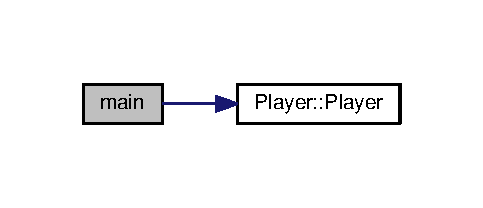
\includegraphics[width=232pt]{Iterator_8cpp_ae66f6b31b5ad750f1fe042a706a4e3d4_cgraph}
\end{center}
\end{figure}



%--- End generated contents ---

% Index
\backmatter
\newpage
\phantomsection
\clearemptydoublepage
\addcontentsline{toc}{chapter}{Index}
\printindex

\end{document}
